\section{Covering Number}
We first introduce the covering number, which is a geometrically intuitive measure of complexity and has been widely used in machine learning theory to analyze generalization error."

\begin{definition}[Covering net and covering number \cite{wang2023enhanced}]
    Let $(\calM, d)$ be a metric space. Consider a bounded subset $\calA \subset \calM$ and let $\vep>0$. A subset $\calN \subseteq \calM$ is called an \textbf{$\vep$-covering net} of $\calA$ if every point in $\calA$ is within a distance $\vep$ of some point of $\calN$, i.e.,
    \begin{equation}
        \forall x \in \calA,\; \exists y \in \calN \;\text{ s.t. } d(x, y) \leq \vep
    \end{equation}
    The smallest cardinality of an $\vep$-covering net of $\calA$ \wrt $d$ is called the \textbf{$\vep$-covering number} of $\calA$ \wrt $d$, denoted by $N(\calA, \vep, d)$, i.e.,
    \[
        N(\calA, \vep, d) \defeq \min \set*{ n \in \mathbb{N} }[ \exists x_1, x_2, \ldots, x_n \in \calM \text{~\,s.t.~} \calA \subseteq \textstyle{\bigcup}_{i=1}^n B_d(x_i, \vep) ],
    \]
    If $\calN \subseteq \calA$, the covering number is denoted by $N_{\text{in}}(\calA, \vep, d)$ and called \textbf{internal covering number}.
    \[
        N_{\text{in}}(\calA, \vep, d) \defeq \min \set*{n \in \bbN}[ \exists x_1, x_2, \ldots, x_n \in \calA \text{~\,s.t.~} \calA \subseteq \textstyle{\bigcup}_{i=1}^n B_d(x_i, \vep) ],
    \]
\end{definition}

You can intuitively understand the covering number as the minimum number of balls with radius $\vep$ needed to cover the set $\calA$ with the metric $d$. The covering number is a measure of the complexity of the set $\calA$.
By definition, $N(\calA, \vep, d) \leq N_{\text{in}}(\calA, \vep, d)$ always holds. For example, when $\calA$ is a doughnut-shaped set, the covering number can be smaller than the internal covering number.

\begin{figure}[H]
    \centering
    \includegraphics[width=6cm]{covering.pdf}
    \caption{Illustration of a covering net}
\end{figure}




\begin{lemma}[Properties of covering number]\label{lem:covering-number-properties}
    Let $(\calM, \norm{\cdot})$ be a normed vector space and $\alpha > 0$. Then, for any bounded subset $\calA \subset \calM$, $\vep > 0$ and $\norm{\cdot}$,
    the following equality holds:
    \begin{align}
        N(\alpha\calA, \vep, \norm{\cdot}) = N(\calA, \vep/\alpha, \norm{\cdot}) = N(\calA, \vep, \alpha \norm{\cdot}) \tag{A} \label{eq:covering-number-properties_A}
    \end{align}
    \begin{align}
        N(\calA, \vep, \norm{\cdot})
        &= N(\alpha\calA, \alpha\vep, \norm{\cdot}) \nonumber\\
        &= N(\calA, \alpha\vep, \alpha \norm{\cdot}) \tag{B} \label{eq:covering-number-properties_B}\\
        &= N(\calA/\alpha, \vep, \alpha \norm{\cdot}) \nonumber
    \end{align}
    
    Let $\calA \subset \calB \subset \calM$, $0 < \vep_1 < \vep_2$, and $\norm{\cdot}_\spadesuit \leq \norm{\cdot}_\clubsuit$. Then the following inequality holds:
    \begin{alignat}{2}
        &N(\calA, \vep, \norm{\cdot}) &&\leq N(\calB, \vep, \norm{\cdot}) \nonumber\\
        &N(\calA, \vep_2, \norm{\cdot}) &&\leq N(\calA, \vep_1, \norm{\cdot}) \tag{C} \label{eq:covering-number-properties_C}\\
        &N(\calA, \vep, \norm{\cdot}_\spadesuit) &&\leq N(\calA, \vep, \norm{\cdot}_\clubsuit) \nonumber
    \end{alignat}
\end{lemma}


\begin{proof}
    \quad\par
     (Proof of \eqref{eq:covering-number-properties_A})
    \begin{itemize}
        \item The first equality holds because expanding (or shrinking) the set $\calA$ by a factor of $\alpha$ is equivalent to shrinking (or expanding) the radius of the balls by a factor of $1/\alpha$ since the covering number only depends on the relative size of the radius and the set.
        \item The second equality holds because $d(x, y) \leq \vep/\alpha$ is equivalent to $\alpha d(x, y) \leq \vep$.
    \end{itemize}
    
    (Proof of \eqref{eq:covering-number-properties_B})
    \begin{itemize}
        \item Since the covering number only depends on the relative size of the radius and the set, expanding (or shrinking) the set $\calA$ and the radius of the balls by a factor of $\alpha$ at the same time does not change the covering number.
        \item The second equality holds because $d(x, y) \leq \vep$ is equivalent to $\alpha d(x, y) \leq \alpha\vep$.
        \item Use the first and second equalities.
    \end{itemize}
    
    (Proof of \eqref{eq:covering-number-properties_C})
    \begin{itemize}
        \item The first inequality holds because the covering number of a larger set is always larger than that of a smaller set.
        \item The second inequality holds because the covering number of a set with a ball of larger radius is always smaller than that of a set with a ball of smaller radius.
        \item If $d_2(x, y) \leq \vep$, then $d_1(x, y) \leq d_2(x, y) \leq \vep$. This implies that if $Q$ is an $\vep$-covering net of $\calA$ with $d_2$, then $Q$ is also an $\vep$-covering net of $\calA$ with $d_1$ and thus
        \begin{align}
            W(\calA, \vep, d_1) \supseteq W(\calA, \vep, d_2)
        \end{align}
        , where $W(\calA, \vep, d)$ represents the set of all $\vep$-covering nets of $\calA$ with $d$.
        Since the covering number is the minimum cardinality of the covering net, it follows that
        \begin{align}
            N(\calA, d_1, \vep)
            &=    \underset{Q \in W(\calA, \vep, d_1)}{\min} \abs{Q}\\
            &\leq \underset{Q \in W(\calA, \vep, d_2)}{\min} \abs{Q}\\
            &=    N(\calA, d_2, \vep)
        \end{align}
    \end{itemize}
\end{proof}




\begin{lemma}[Covering number of normalized norm]
    \begin{equation}
        N(\calA, \vep, \norm{\cdot}_p) = N(\calA, \vep/m^{\frac1p}, \norm{\cdot}_{p,m})
    \end{equation}
\end{lemma}


\begin{proof}
    From the definition of normalized $p$-norm, $\norm{a - a'}_p \leq \vep$ and $\norm{a - a'}_{p,m} \leq \vep/m^{\frac1p}$ is equivalent, thus the equation holds.
\end{proof}





\begin{lemma}[Inequality of covering numbers with different norms]\label{lem:covering-number-inequality-1}
    The following inequality holds for any $\vep > 0$ and any bounded subset $\calA \subset \bbR^{m}$:
    \begin{alignat}{3}
        N(\calA, \vep, \norm{\cdot}_{\infty}) &\leq N(\calA, \vep, \norm{\cdot}_{q}) &&\leq N(\calA, \vep, \norm{\cdot}_{p}) &&\leq N(\calA, \vep, \norm{\cdot}_{1})\\
        N(\calA, \vep, \norm{\cdot}_{1,n}) &\leq N(\calA, \vep, \norm{\cdot}_{p,n}) &&\leq N(\calA, \vep, \norm{\cdot}_{q,n}) &&\leq N(\calA, \vep, \norm{\cdot}_{\infty,n})
    \end{alignat}
    where $1 \leq p \leq q < \infty$.
\end{lemma}


\begin{proof}
    Use the Lemma \ref{lem:inequality-p-norms} and the inequality \eqref{eq:covering-number-properties_C} in Lemma \ref{lem:covering-number-properties}.
\end{proof}

\begin{remark}
    From the properties of $p$-norm, for any two points $\bs{x}, \bs{y} \in \bbR^{m}$ and $1 \leq p \leq q < \infty$, you have $\norm{\bs{x}-\bs{y}}_{\infty} \leq \norm{\bs{x}-\bs{y}}_{q} \leq \norm{\bs{x}-\bs{y}}_{p} \leq \norm{\bs{x}-\bs{y}}_{1}$.
    This implies that $B_{1}(\bs{x}, \vep) \subset B_{p}(\bs{x}, \vep) \subset B_{q}(\bs{x}, \vep) \subset B_{\infty}(\bs{x}, \vep)$.
    This is also obvious from Fig. \ref{fig:p-norm-contours_1}.
    From this fact, you can see that you need more balls to cover $\calA$ with the $q$-norm ball than with the $p$-norm ball.
\end{remark}


\begin{figure}[H]
    \centering
    \includegraphics[width=8cm]{p_norm_contours_1.pdf}
    \caption{The contours of $p$-norm balls with $\vep = 1$ in $\bbR^{2}$ for $p = 1, 2, 3, \infty$.}
    \label{fig:p-norm-contours_1}
\end{figure}





\begin{lemma}\label{lem:covering-number-inequality-2}
    The following inequality holds for any $\vep > 0$, some subset $\calA \subset \bbR^{m}$, and $1 \leq r < p$:
    \begin{equation}
        N(\calA, \vep, \norm{\cdot}_p) \leq N(\calA, \vep, \norm{\cdot}_r) \leq N(\calA, \vep, m^{(1/r - 1/p)}\norm{\cdot}_p)
    \end{equation}
\end{lemma}


\begin{proof}
    From Lemma \ref{lem:inequality-p-norms}, it holds that $\norm{\bs{x}}_p \leq \norm{\bs{x}}_r \leq m^{(1/r - 1/p)}\norm{\bs{x}}_p$ for $1 \leq r < p$ and $\bs{x} \in \bbR^n$. Thus, you can use the last inequality in \eqref{eq:covering-number-properties_C} in Lemma \ref{lem:covering-number-properties}.
\end{proof}

\begin{example}
    When $p = \infty$ and $r = 1$, you have $N(\calA, \vep, \norm{\cdot}_{\infty}) \leq N(\calA, \vep, \norm{\cdot}_{1}) \leq N(\calA, \vep, m\,\norm{\cdot}_{\infty}) = N(\calA, \vep/m, \norm{\cdot}_{\infty})$.
    The Fig. \ref{fig:p-norm-contours_2} illustrates the inequality between covering numbers visually.
    The Fig. \ref{fig:p-norm-contours_2} shows the contours of $1$-norm ball with $\vep = 1$ and $\infty$-norm balls with $\vep = 1/2, 1$ in $\bbR^{2}$. You can see that $B_{\infty}(\bs{x}, \vep/2) \subset B_{1}(\bs{x}, \vep)$. In $\bbR^{m}$, you have $B_{\infty}(\bs{x}, \vep/m) \subset B_{1}(\bs{x}, \vep)$. Thus, you need more balls to cover $\calA$ with the $\infty$-norm ball with radius $\vep/m$ than with the $1$-norm ball with radius $\vep$.
\end{example}

\begin{figure}[H]
    \centering
    \includegraphics[width=8cm]{p_norm_contours_2.pdf}
    \caption{The contours of $1$-norm ball with $\vep = 1$ in $\bbR^{2}$ and $\infty$-norm balls with $\vep = 1/2, 1$ in $\bbR^{2}$}
    \label{fig:p-norm-contours_2}
\end{figure}






The following lemma enables us to employ the covering number of one metric space to bound the covering number of another metric space. (Lemma 5 in Ref.~\cite{barthel2018fundamental}.)

\begin{lemma}[Covering numbers of two metric spaces \cite{wang2023enhanced}]\label{lem:2-covering-number}
    Let $\left(\calM_{1}, d_{1}\right)$ and $\left(\calM_{2}, d_{2}\right)$ be two metric spaces and $f: \calM_{1} \rightarrow \calM_{2}$ be $K$-Lipschitz such that
    \begin{equation}
        d_{2}(f(x), f(y)) \leq K\, d_{1}(x, y), \forall x, y \in \calM_{1}
    \end{equation}
    where $K$ is a constant. Then, you can use the covering number of a bounded subset $\calA_1 \subset \calM_1$ with $d_1$ to bound the covering number of a bounded subset $f(\calA_1) \subset \calM_2$ with $d_2$ as
    \begin{equation}
        N\left(f(\calA_1), \vep, d_{2}\right) \leq N\left(\calA_{1}, \vep/K, d_{1}\right)
    \end{equation}
\end{lemma}



\begin{proof}
    Let $\calQ_1$ be an $\vep/K$-covering net for $\calA_1$ with $d_1$, that is, $\forall x \in \calA_1,\,\exists y \in \calQ_1$ such that $d_1(x, y) \leq \vep/K$.
    Since, for any $X\in f(\calA_1)$, there exists $x\in \calA_1$ such that $X = f(x)$, and there exists $y \in \calQ_1$ such that $d_1(x, y) \leq \vep/K$, 
    it follows $\forall X \in f(\calA_1),\,\exists Y = f(y) \in f(\calQ_1)$ such that $d_2(X, Y) \leq$ $K d_1(x, y) \leq \vep$ (the first inequality is due to assumption of $K$-Lipschitzness of $f$). Therefore, $f(\calQ_1)$ is an $\vep$-covering net of $f(\calA_1)$ with $d_2$.
    It implies that if $Q_1$ is an $\vep/K$-covering net of $\calA_1$ with $d_1$, then $f(Q_1)$ is an $\vep$-covering net of $f(\calA_1)$ with $d_2$, and thus
    \begin{align}
        W(f(\calA_1), \vep, d_2) \supseteq \set{f(\calQ_1)}[\calQ_1 \in W(\calA_1, \vep/K, d_1)]\label{eq:covering-net-include}
    \end{align}
    , where $W(f(\calA_1), \vep, d_2)$ is the set of all $\vep$-covering nets of $f(\calA_1)$ with $d_2$ and $W(\calA_1, \vep/K, d_1)$ is the set of all $\vep/K$-covering nets of $\calA_1$ with $d_1$.
    Since the covering number is the minimum cardinality of the covering net, it follows that
    \begin{align}
        N(f(\calA_1), d_2, \vep)
        &=    \underset{\calQ_2 \in W(f(\calA_1), \vep, d_2)}{\min} \abs{\calQ_2}\\
        &\overset{(a)}{\leq}
        \underset{\calQ_1 \in W(\calA_1, \vep/K, d_1)}{\min} \abs{f(\calQ_1)}\\
        &\overset{(b)}{\leq}
        \underset{\calQ_1 \in W(\calA_1, \vep/K, d_1)}{\min} \abs{\calQ_1}\\
        &=    N(\calA_1, d_1, \vep/K)
    \end{align}
    Equality in (a) holds if the equality in \eqref{eq:covering-net-include} holds, and equality in (b) holds if $f$ is injective.
\end{proof}

\begin{example}
    Let $\calA_1 := [0, 1]$ and $f: \calA_1 \ni x \mapsto \pi x \subset [0, \pi] = f(\calA_1)$, then $f$ is $K$-Lipschitz with $K = \pi$. Then, $N(\calA_1, \vep, \norm{\cdot}) = \lceil\frac{1}{2\vep}\rceil$ and $N(f(\calA_1), \vep, \norm{\cdot}) = \lceil\frac{\pi}{2\vep}\rceil$. Thus, $N(f(\calA_1), \vep, \norm{\cdot}) = \lceil\frac{\pi}{2\vep}\rceil \leq \lceil\frac{\pi}{2\vep}\rceil = N(\calA_1, \vep/\pi, \norm{\cdot})$.
\end{example}

\begin{example}
    Let $\calA_1 := [0, 1]$ and $f: \calA_1 \ni x \mapsto \sin(\pi x) \subset [0, 1] = f(\calA_1)$, then $f$ is $K$-Lipschitz with $K = \pi$. Then, $N(\calA_1, \vep, \norm{\cdot}) = \lceil\frac{1}{2\vep}\rceil$ and $N(f(\calA_1), \vep, \norm{\cdot}) = \lceil\frac{1}{2\vep}\rceil$. Thus, $N(f(\calA_1), \vep, \norm{\cdot}) = \lceil\frac{1}{2\vep}\rceil \leq \lceil\frac{\pi}{2\vep}\rceil = N(\calA_1, \vep/\pi, \norm{\cdot})$.
\end{example}








\begin{definition}[Packing]
    Let $(\calM, d)$ be a metric space. Consider a bounded subset $\calA \subset \calM$ and let $\vep>0$. A subset $\calP \subseteq \calA$ is called an \textbf{$\vep$-packing} of $\calA$ if every pair of distinct points in $\calP$ is separated by a distance greater than $\vep$, i.e.,
    \begin{equation}
        \forall x, y \in \calP,\; d(x, y)>\vep .
    \end{equation}
    The largest possible cardinality of an $\vep$-packing of $\calA$ \wrt $d$ is called the \textbf{$\vep$-packing number} of $\calA$ \wrt $d$, denoted by $M(\calA, \vep, d)$, i.e.,
    \begin{align}
        M(\calA, \vep, d)
        &\defeq \max \set{|\calP| : \text{$\calP$ is an $\vep$-packing of $\calA$}}\\
        &\defeq \max \set*{ n \in \mathbb{N} }[ \exists x_1, x_2, \ldots, x_n \in \calA \text{~\,s.t.~} \forall i, j \in [n],\, i \neq j \Rightarrow d(x_i, x_j) > \vep ]
    \end{align}
    , where $[n] \defeq \set{1, 2, \ldots, n}$.
\end{definition}



\begin{figure}[H]
    \centering
    \includegraphics[width=14cm]{packing.pdf}
    \caption{(Left) Illustration of a packing. All points in the set $\calP$ are separated by a distance greater than $\vep$. You can add more points to $\calP$ without violating the condition because there is still some space not covered by the balls.
    (Right) If we consider the balls with radius $\vep/2$ centered at the points in $\calP$, then the balls are disjoint.}
\end{figure}





\begin{lemma}[Inequality between covering number and packing number]
    Let $\calA \subset \bbR^{m}$ be a bounded subset and $\vep > 0$. Then, the following inequality holds:
    \begin{equation}
        N(\calA, \vep, d) \leq N_{\text{in}}(\calA, \vep, d) \leq M(\calA, \vep, d) \leq N(\calA, \vep/2, d)
    \end{equation}
\end{lemma}



\begin{proof}
    \quad\par
    The first inequality is trivial from the definition of the covering number.
    
    (Proof of the second inequality)\\
    If $\calP$ is an $\vep$-packing of $\calA$ such that $|\calP| = M(\calA,\vep,d)$, for any point $a \in \calA \backslash \calP$, the set $\calP \cup\{a\}$ is not an $\vep$-packing of $\calA$. Namely, for any $a \in \calA$ there exists $p \in \calP$ such that $d(a, p) \leq \vep$. Hence, $\calP$ is an internal $\vep$-covering net of $\calA$, and so $N_{\text{in}}(\calA, \vep, d) \leq |\calP|$.\\
    
    (Proof of the third inequality)\\
    Let $\calB$ be an $\vep/2$-covering net of $\calA$ such that $|\calB| = N(\calA, \vep/2, d)$. Let $\calP$ be any $\vep$-packing of $\calA$. Since any two points in $\calP$ are separated by a distance greater than $\vep$ (i.e., $d(p, p') > \vep$ for any $p, p' \in \calP$),
    for any $b \in \calB$, there exists at most one $p \in \calP$ such that $d(b, p) \leq \vep/2$. Hence, $|\calP| \leq |\calB|$, and so $M(\calA, \vep, d) \leq N(\calA, \vep/2, d)$.
\end{proof}





\begin{lemma}[covering number of a norm ball]\label{lem:covering-number-norm-ball}
    Let $\bs{x} \in \bbR^{m}$, $0 < \vep \leq R$, and $\norm{\cdot}$ be any norm on $\bbR^{m}$.
    Then, the covering number of the norm ball $B(\bs{x},R,\norm{\cdot})$ is bounded as
    \begin{equation}
    \left(\frac{R}{\vep}\right)^m \leq N(B(\bs{x},R,\norm{\cdot}), \vep, \norm{\cdot})\leq \left( 1 + \frac{2R}{\vep}\right)^m \leq \left(\frac{3R}{\vep}\right)^m.
    \end{equation}
\end{lemma}


\begin{proof}
    We denote the volume of the unit ball in $\bbR^{m}$ as $V$. Then, the volume of $B(\bs{x},r,\norm{\cdot})$ is $r^m V$.\\
    (Proof of the first inequality)\\
    Let $\calN$ be an $\vep$-covering net of $B(\bs{x},R,\norm{\cdot})$ such that $|\calN| = N(B(\bs{x},R,\norm{\cdot}), \vep, \norm{\cdot})$.
    Then, since $B(\bs{x},R,\norm{\cdot}) \subset \cup_{n \in \calN} B(n,\vep,\norm{\cdot})$, we have
    \begin{align}
        \mathrm{Volume}(B(\bs{x},R,\norm{\cdot})) \leq \mathrm{Volume}(\cup_{n \in \calN} B(n,\vep,\norm{\cdot})) \leq \sum_{n \in \calN}\mathrm{Volume}(B(n,\vep,\norm{\cdot})).
    \end{align}
    Thus, $R^m V \leq |\calN| \times \vep^m V$, and so $(R/\vep)^m \leq |\calN|$.\\
    
    (Proof of the second inequality)\\
    Let $\calP$ be an $\vep$-packing of $B(\bs{x},R,\norm{\cdot})$ such that $|\calP| = M(B(\bs{x},R,\norm{\cdot}), \vep, \norm{\cdot})$.
    Then, since the balls $B(p,\vep/2,\norm{\cdot})$ are disjoint for $p \in \calP$ and all these balls are contained in $B(\bs{x},R+\vep/2,\norm{\cdot})$, we have
    \begin{align}
        \mathrm{Volume}(\cup_{p \in \calP} B(p,\vep/2,\norm{\cdot}))
        = \sum_{p \in \calP} \mathrm{Volume}(B(p,\vep/2,\norm{\cdot}))
        \leq \mathrm{Volume}(B(\bs{x},R+\vep/2,\norm{\cdot})).
    \end{align}
    Thus, $|\calP| \times (\vep/2)^m V \leq (\vep/2+R)^m V$, and so $|\calP| \leq (1 + 2R/\vep)^m$. The last inequality holds because $1 + 2R/\vep \leq 3R/\vep$. Finally, we use the fact that $|\calN| \leq |\calP|$.
\end{proof}








\begin{lemma}[covering number of a hypercube]
    The covering number of a hypercube $\Theta \defeq \set{(\theta_1, \theta_2,\ldots, \theta_m)}[\theta_i \in [a_i, a_i + c_i],\, a_i,c_i \in \bbR] \subset \bbR^m$ w.r.t. the $\infty$-norm is equal to
    \begin{equation}
        N(\Theta,\, \vep,\norm{\cdot}_{\infty}) = \prod_{i=1}^{m} \left\lceil\frac{c_{i}}{2\vep}\right\rceil
    \end{equation}
\end{lemma}


The $\infty$-norm ball is a hypercube with side length $2\vep$. For each side of the hypercube $\Theta$, you need $\lceil\frac{c_{i}}{2\vep}\rceil$ hypercubes to cover the side. Thus, you need $\prod_{i=1}^{m} \lceil\frac{c_{i}}{2\vep}\rceil$ hypercubes to cover the hypercube $\Theta$.
\begin{figure}[H]
    \centering
    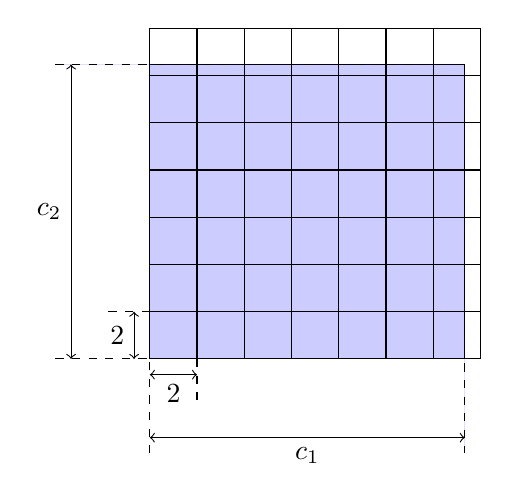
\begin{tikzpicture}[scale=2]
        \draw[fill=blue!20] (0,0) -- (0,1.87) -- (2,1.87) -- (2,0) -- (0,0);
        \draw[dashed] (-0.6,0) -- (0,0);
        \draw[dashed] (0,-0.6) -- (0,0);
        \draw[dashed] (0, 0.3) -- (-0.3,0.3);
        \draw[dashed] (0.3, 0) -- (0.3,-0.3);
        \draw[dashed,fill=blue] (-0.6,1.87) -- (2,1.87);
        \draw[dashed,fill=blue] (2,1.87) -- (2,-0.6);
        \draw[] (0,0)   -- (0,  2.1);
        \draw[] (0,0)   -- (2.1,  0);
        \draw[] (0.3,0) -- (0.3,2.1);
        \draw[] (0.6,0) -- (0.6,2.1);
        \draw[] (0.9,0) -- (0.9,2.1);
        \draw[] (1.2,0) -- (1.2,2.1);
        \draw[] (1.5,0) -- (1.5,2.1);
        \draw[] (1.8,0) -- (1.8,2.1);
        \draw[] (2.1,0) -- (2.1,2.1);
        \draw[] (0,0.3) -- (2.1,0.3);
        \draw[] (0,0.6) -- (2.1,0.6);
        \draw[] (0,0.9) -- (2.1,0.9);
        \draw[] (0,1.2) -- (2.1,1.2);
        \draw[] (0,1.5) -- (2.1,1.5);
        \draw[] (0,1.8) -- (2.1,1.8);
        \draw[] (0,2.1) -- (2.1,2.1);
        \draw[] (0,2.1) -- (2.1,2.1);
        % we add the length of the side of the hypercube to the figure
        \draw[<->] (0, -0.5) -- (2, -0.5) node[midway, below]{$c_1$};
        \draw[<->] (-0.5, 0) -- (-0.5, 1.87) node[midway, left]{$c_2$};
        % we add the length of the side of the ball to the figure
        \draw[<->] (0, -0.1) -- (0.3, -0.1) node[midway, below]{$2\vep$};
        \draw[<->] (-0.1, 0) -- (-0.1, 0.3) node[midway, left]{$2\vep$};
    \end{tikzpicture}
    \caption{$\vep$-covering net of a hypercube $\Theta \subset \bbR^{2}$ w.r.t. $\norm{\cdot}_{\infty}$}
    \label{fig:covering-number-hypercube}
\end{figure}







In the following, we consider $\Theta \defeq \set{(\theta_1, \theta_2,\ldots, \theta_m)}[\theta_i \in [a_i, a_i + c_i],\, a_i,c_i \in \bbR] \subset \bbR^m$ in which some parameters have correlations, \ie $\theta_i = \theta_j$ for some $i \neq j$. We can derive the covering number of $\Theta$ as follows.


\begin{lemma}[covering number of a hypercube with some correlations]\label{lem:covering-number-correlations}
    Let $\Theta \defeq \set{(\theta_1, \theta_2,\ldots, \theta_m)}[\theta_i \in [a_i, a_i + c_i],\, a_i,c_i \in \bbR] \subset \bbR^m$ in which some parameters have correlations, \ie $\theta_1 = k\,\theta_2$ with $k \in \bbR$.
    Then, the covering number of $\Theta$ \wrt the $\infty$-norm is upper bounded as
    \begin{equation}
        N(\Theta,\, \vep,\norm{\cdot}_{\infty}) \leq \prod_{j=1}^{T} \left\lceil\frac{c_{i_j}}{2\vep}\right\rceil
    \end{equation}
    , where $T$ is the number of independent parameters. $c_{i_j}$ is the largest one in those of dependent parameters.
\end{lemma}



\begin{proof}
    You can understand Lemma \ref{lem:covering-number-correlations} from the following example in $\bbR^{3}$.
    When all parameters are independent, then the covering number of $\Theta$ is equal to $\left\lceil\frac{c_1}{2\vep}\right\rceil \times \left\lceil\frac{c_2}{2\vep}\right\rceil \times \left\lceil\frac{c_3}{2\vep}\right\rceil$. However, when $\theta_2 = \theta_3$, $\Theta$ is a plane in $\bbR^{3}$, and you only need to consider the covering number of the plane. As shown in Fig. \ref{fig:covering-number-hypercube-correlations}, you can align the $\infty$-norm ball with the plane, and see that you can cover the plane with the same covering number of the hypercube $[a_1, a_1 + c_1] \times [a_2, a_2+ c_2]$ in $\bbR^{2}$, which is $\left\lceil\frac{c_1}{2\vep}\right\rceil \times \left\lceil\frac{c_2}{2\vep}\right\rceil$.
    \begin{figure}[H]
    \centering
    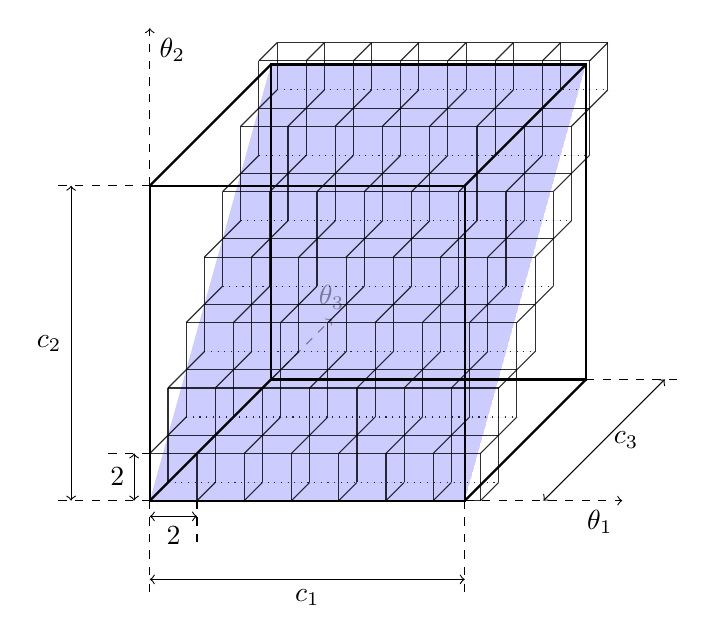
\begin{tikzpicture}[scale=2]
        % Define the cube's vertices
        \coordinate (A) at (0,0,0);
        \coordinate (B) at (2,0,0);
        \coordinate (C) at (2,2,0);
        \coordinate (D) at (0,2,0);
        \coordinate (E) at (0,0,2);
        \coordinate (F) at (2,0,2);
        \coordinate (G) at (2,2,2);
        \coordinate (H) at (0,2,2);

        % Draw the shaded area under the hypercube
        \begin{scope}
            \clip (D) -- (E) -- (F) -- (C);
            \fill[blue!20] (D) -- (E) -- (F) -- (C);
        \end{scope}
        
        % Draw the front face
        \draw[thick] (A) -- (B) -- (C) -- (D) -- cycle;

        % Draw the back face
        \draw[thick] (E) -- (F) -- (G) -- (H) -- cycle;

        % Draw the connecting edges
        \draw[thick] (A) -- (E);
        \draw[thick] (B) -- (F);
        \draw[thick] (C) -- (G);
        \draw[thick] (D) -- (H);
    
        % Label the axes
        \draw[->, dashed] (0,0,2) -- (3,0,2) node[anchor=north east] {$\theta_1$};
        \draw[->, dashed] (0,0,2) -- (0,3,2) node[anchor=north west] {$\theta_2$};
        \draw[->, dashed,opacity=0.4] (0,0,0) -- (0,0,-1) node[anchor=south] {$\theta_3$};
        
        \draw[<->] (0,-0.1,2)  -- (0.3,-0.1,2) node[midway, below]{$2\vep$};
        \draw[<->] (-0.1,0,2)  -- (-0.1,0.3,2) node[midway, left]{$2\vep$};
        \draw[dashed] (0,0.3,2)  -- (-0.3,0.3,2);
        \draw[dashed] (0.3,0,2)  -- (0.3,-0.3,2);
        
        \draw[<->] (0,-0.5,2)  -- (2,-0.5,2) node[midway, below]{$c_1$};
        \draw[<->] (-0.5,0,2)  -- (-0.5,2,2) node[midway, left]{$c_2$};
        \draw[<->] (2.5,0,2)   -- (2.5,0,0)  node[midway, right]{$c_3$};
        \draw[dashed] (0,0,2)  -- (-0.6,0,2);
        \draw[dashed] (0,2,2)  -- (-0.6,2,2);
        \draw[dashed] (0,0,2)  -- (0,-0.6,2);
        \draw[dashed] (2,0,2)  -- (2,-0.6,2);
        \draw[dashed] (2,0,0)  -- (2.6,0,0);
        
        % Draw the p-norm balls which cover the hypercube
        \draw[opacity=0.8, fill=blue!50] (0.3,0,2)   -- (0.3,0.3,2);
        \draw[opacity=0.8, fill=blue!50] (0.3,0,2)   -- (0.3,0,1.7);
        \draw[opacity=0.8, fill=blue!50] (0.6,0,2)   -- (0.6,0.3,2);
        \draw[opacity=0.8, fill=blue!50] (0.6,0,2)   -- (0.6,0,1.7);
        \draw[opacity=0.8, fill=blue!50] (0.9,0,2)   -- (0.9,0.3,2);
        \draw[opacity=0.8, fill=blue!50] (0.9,0,2)   -- (0.9,0,1.7);
        \draw[opacity=0.8, fill=blue!50] (1.2,0,2)   -- (1.2,0.3,2);
        \draw[opacity=0.8, fill=blue!50] (1.2,0,2)   -- (1.2,0,1.7);
        \draw[opacity=0.8, fill=blue!50] (1.5,0,2)   -- (1.5,0.3,2);
        \draw[opacity=0.8, fill=blue!50] (1.5,0,2)   -- (1.5,0,1.7);
        \draw[opacity=0.8, fill=blue!50] (1.8,0,2)   -- (1.8,0.3,2);
        \draw[opacity=0.8, fill=blue!50] (1.8,0,2)   -- (1.8,0,1.7);
        \draw[opacity=0.8, fill=blue!50] (2.1,0,2)   -- (2.1,0.3,2);
        \draw[opacity=0.8, fill=blue!50] (2.1,0,2)   -- (2.1,0,1.7);
        
        \draw[opacity=0.8, fill=blue!50] (0,0.3,2)   -- (0,0.3,1.4);
        \draw[opacity=0.8, fill=blue!50] (0.3,0.3,2) -- (0.3,0.3,1.4);
        \draw[opacity=0.8, fill=blue!50] (0.6,0.3,2) -- (0.6,0.3,1.4);
        \draw[opacity=0.8, fill=blue!50] (0.9,0.3,2) -- (0.9,0.3,1.4);
        \draw[opacity=0.8, fill=blue!50] (1.2,0.3,2) -- (1.2,0.3,1.4);
        \draw[opacity=0.8, fill=blue!50] (1.5,0.3,2) -- (1.5,0.3,1.4);
        \draw[opacity=0.8, fill=blue!50] (1.8,0.3,2) -- (1.8,0.3,1.4);
        \draw[opacity=0.8, fill=blue!50] (2.1,0.3,2) -- (2.1,0.3,1.4);
        \draw[opacity=0.8, fill=blue!50] (0,0,1.7)   -- (0,0.6,1.7);
        \draw[opacity=0.8, fill=blue!50] (0.3,0,1.7) -- (0.3,0.6,1.7);
        \draw[opacity=0.8, fill=blue!50] (0.6,0,1.7) -- (0.6,0.6,1.7);
        \draw[opacity=0.8, fill=blue!50] (0.9,0,1.7) -- (0.9,0.6,1.7);
        \draw[opacity=0.8, fill=blue!50] (1.2,0,1.7) -- (1.2,0.6,1.7);
        \draw[opacity=0.8, fill=blue!50] (1.5,0,1.7) -- (1.5,0.6,1.7);
        \draw[opacity=0.8, fill=blue!50] (1.8,0,1.7) -- (1.8,0.6,1.7);
        \draw[opacity=0.8, fill=blue!50] (2.1,0,1.7) -- (2.1,0.6,1.7);
        \draw[opacity=0.8, fill=blue!50] (0,0.6,1.7) -- (0,0.6,1.1);
        \draw[opacity=0.8, fill=blue!50] (0.3,0.6,1.7) -- (0.3,0.6,1.1);
        \draw[opacity=0.8, fill=blue!50] (0.6,0.6,1.7) -- (0.6,0.6,1.1);
        \draw[opacity=0.8, fill=blue!50] (0.9,0.6,1.7) -- (0.9,0.6,1.1);
        \draw[opacity=0.8, fill=blue!50] (1.2,0.6,1.7) -- (1.2,0.6,1.1);
        \draw[opacity=0.8, fill=blue!50] (1.5,0.6,1.7) -- (1.5,0.6,1.1);
        \draw[opacity=0.8, fill=blue!50] (1.8,0.6,1.7) -- (1.8,0.6,1.1);
        \draw[opacity=0.8, fill=blue!50] (2.1,0.6,1.7) -- (2.1,0.6,1.1);
        \draw[opacity=0.8, fill=blue!50] (0,0.3,1.4) -- (0,0.9,1.4);
        \draw[opacity=0.8, fill=blue!50] (0.3,0.3,1.4) -- (0.3,0.9,1.4);
        \draw[opacity=0.8, fill=blue!50] (0.6,0.3,1.4) -- (0.6,0.9,1.4);
        \draw[opacity=0.8, fill=blue!50] (0.9,0.3,1.4) -- (0.9,0.9,1.4);
        \draw[opacity=0.8, fill=blue!50] (1.2,0.3,1.4) -- (1.2,0.9,1.4);
        \draw[opacity=0.8, fill=blue!50] (1.5,0.3,1.4) -- (1.5,0.9,1.4);
        \draw[opacity=0.8, fill=blue!50] (1.8,0.3,1.4) -- (1.8,0.9,1.4);
        \draw[opacity=0.8, fill=blue!50] (2.1,0.3,1.4) -- (2.1,0.9,1.4);
        \draw[opacity=0.8, fill=blue!50] (0,0.9,1.4) -- (0,0.9,0.8);
        \draw[opacity=0.8, fill=blue!50] (0.3,0.9,1.4) -- (0.3,0.9,0.8);
        \draw[opacity=0.8, fill=blue!50] (0.6,0.9,1.4) -- (0.6,0.9,0.8);
        \draw[opacity=0.8, fill=blue!50] (0.9,0.9,1.4) -- (0.9,0.9,0.8);
        \draw[opacity=0.8, fill=blue!50] (1.2,0.9,1.4) -- (1.2,0.9,0.8);
        \draw[opacity=0.8, fill=blue!50] (1.5,0.9,1.4) -- (1.5,0.9,0.8);
        \draw[opacity=0.8, fill=blue!50] (1.8,0.9,1.4) -- (1.8,0.9,0.8);
        \draw[opacity=0.8, fill=blue!50] (2.1,0.9,1.4) -- (2.1,0.9,0.8);
        \draw[opacity=0.8, fill=blue!50] (0,0.6,1.1) -- (0,1.2,1.1);
        \draw[opacity=0.8, fill=blue!50] (0.3,0.6,1.1) -- (0.3,1.2,1.1);
        \draw[opacity=0.8, fill=blue!50] (0.6,0.6,1.1) -- (0.6,1.2,1.1);
        \draw[opacity=0.8, fill=blue!50] (0.9,0.6,1.1) -- (0.9,1.2,1.1);
        \draw[opacity=0.8, fill=blue!50] (1.2,0.6,1.1) -- (1.2,1.2,1.1);
        \draw[opacity=0.8, fill=blue!50] (1.5,0.6,1.1) -- (1.5,1.2,1.1);
        \draw[opacity=0.8, fill=blue!50] (1.8,0.6,1.1) -- (1.8,1.2,1.1);
        \draw[opacity=0.8, fill=blue!50] (2.1,0.6,1.1) -- (2.1,1.2,1.1);
        \draw[opacity=0.8, fill=blue!50] (0,1.2,1.1) -- (0,1.2,0.5);
        \draw[opacity=0.8, fill=blue!50] (0.3,1.2,1.1) -- (0.3,1.2,0.5);
        \draw[opacity=0.8, fill=blue!50] (0.6,1.2,1.1) -- (0.6,1.2,0.5);
        \draw[opacity=0.8, fill=blue!50] (0.9,1.2,1.1) -- (0.9,1.2,0.5);
        \draw[opacity=0.8, fill=blue!50] (1.2,1.2,1.1) -- (1.2,1.2,0.5);
        \draw[opacity=0.8, fill=blue!50] (1.5,1.2,1.1) -- (1.5,1.2,0.5);
        \draw[opacity=0.8, fill=blue!50] (1.8,1.2,1.1) -- (1.8,1.2,0.5);
        \draw[opacity=0.8, fill=blue!50] (2.1,1.2,1.1) -- (2.1,1.2,0.5);
        \draw[opacity=0.8, fill=blue!50] (0,0.9,0.8) -- (0,1.5,0.8);
        \draw[opacity=0.8, fill=blue!50] (0.3,0.9,0.8) -- (0.3,1.5,0.8);
        \draw[opacity=0.8, fill=blue!50] (0.6,0.9,0.8) -- (0.6,1.5,0.8);
        \draw[opacity=0.8, fill=blue!50] (0.9,0.9,0.8) -- (0.9,1.5,0.8);
        \draw[opacity=0.8, fill=blue!50] (1.2,0.9,0.8) -- (1.2,1.5,0.8);
        \draw[opacity=0.8, fill=blue!50] (1.5,0.9,0.8) -- (1.5,1.5,0.8);
        \draw[opacity=0.8, fill=blue!50] (1.8,0.9,0.8) -- (1.8,1.5,0.8);
        \draw[opacity=0.8, fill=blue!50] (2.1,0.9,0.8) -- (2.1,1.5,0.8);
        \draw[opacity=0.8, fill=blue!50] (0,1.5,0.8) -- (0,1.5,0.2);
        \draw[opacity=0.8, fill=blue!50] (0.3,1.5,0.8) -- (0.3,1.5,0.2);
        \draw[opacity=0.8, fill=blue!50] (0.6,1.5,0.8) -- (0.6,1.5,0.2);
        \draw[opacity=0.8, fill=blue!50] (0.9,1.5,0.8) -- (0.9,1.5,0.2);
        \draw[opacity=0.8, fill=blue!50] (1.2,1.5,0.8) -- (1.2,1.5,0.2);
        \draw[opacity=0.8, fill=blue!50] (1.5,1.5,0.8) -- (1.5,1.5,0.2);
        \draw[opacity=0.8, fill=blue!50] (1.8,1.5,0.8) -- (1.8,1.5,0.2);
        \draw[opacity=0.8, fill=blue!50] (2.1,1.5,0.8) -- (2.1,1.5,0.2);
        \draw[opacity=0.8, fill=blue!50] (0,1.2,0.5) -- (0,1.8,0.5);
        \draw[opacity=0.8, fill=blue!50] (0.3,1.2,0.5) -- (0.3,1.8,0.5);
        \draw[opacity=0.8, fill=blue!50] (0.6,1.2,0.5) -- (0.6,1.8,0.5);
        \draw[opacity=0.8, fill=blue!50] (0.9,1.2,0.5) -- (0.9,1.8,0.5);
        \draw[opacity=0.8, fill=blue!50] (1.2,1.2,0.5) -- (1.2,1.8,0.5);
        \draw[opacity=0.8, fill=blue!50] (1.5,1.2,0.5) -- (1.5,1.8,0.5);
        \draw[opacity=0.8, fill=blue!50] (1.8,1.2,0.5) -- (1.8,1.8,0.5);
        \draw[opacity=0.8, fill=blue!50] (2.1,1.2,0.5) -- (2.1,1.8,0.5);
        \draw[opacity=0.8, fill=blue!50] (0,1.8,0.5) -- (0,1.8,-0.1);
        \draw[opacity=0.8, fill=blue!50] (0.3,1.8,0.5) -- (0.3,1.8,-0.1);
        \draw[opacity=0.8, fill=blue!50] (0.6,1.8,0.5) -- (0.6,1.8,-0.1);
        \draw[opacity=0.8, fill=blue!50] (0.9,1.8,0.5) -- (0.9,1.8,-0.1);
        \draw[opacity=0.8, fill=blue!50] (1.2,1.8,0.5) -- (1.2,1.8,-0.1);
        \draw[opacity=0.8, fill=blue!50] (1.5,1.8,0.5) -- (1.5,1.8,-0.1);
        \draw[opacity=0.8, fill=blue!50] (1.8,1.8,0.5) -- (1.8,1.8,-0.1);
        \draw[opacity=0.8, fill=blue!50] (2.1,1.8,0.5) -- (2.1,1.8,-0.1);
        \draw[opacity=0.8, fill=blue!50] (0,1.5,0.2) -- (0,2.1,0.2);
        \draw[opacity=0.8, fill=blue!50] (0.3,1.5,0.2) -- (0.3,2.1,0.2);
        \draw[opacity=0.8, fill=blue!50] (0.6,1.5,0.2) -- (0.6,2.1,0.2);
        \draw[opacity=0.8, fill=blue!50] (0.9,1.5,0.2) -- (0.9,2.1,0.2);
        \draw[opacity=0.8, fill=blue!50] (1.2,1.5,0.2) -- (1.2,2.1,0.2);
        \draw[opacity=0.8, fill=blue!50] (1.5,1.5,0.2) -- (1.5,2.1,0.2);
        \draw[opacity=0.8, fill=blue!50] (1.8,1.5,0.2) -- (1.8,2.1,0.2);
        \draw[opacity=0.8, fill=blue!50] (2.1,1.5,0.2) -- (2.1,2.1,0.2);
        \draw[opacity=0.8, fill=blue!50] (0,2.1,0.2) -- (0,2.1,-0.1);
        \draw[opacity=0.8, fill=blue!50] (0.3,2.1,0.2) -- (0.3,2.1,-0.1);
        \draw[opacity=0.8, fill=blue!50] (0.6,2.1,0.2) -- (0.6,2.1,-0.1);
        \draw[opacity=0.8, fill=blue!50] (0.9,2.1,0.2) -- (0.9,2.1,-0.1);
        \draw[opacity=0.8, fill=blue!50] (1.2,2.1,0.2) -- (1.2,2.1,-0.1);
        \draw[opacity=0.8, fill=blue!50] (1.5,2.1,0.2) -- (1.5,2.1,-0.1);
        \draw[opacity=0.8, fill=blue!50] (1.8,2.1,0.2) -- (1.8,2.1,-0.1);
        \draw[opacity=0.8, fill=blue!50] (2.1,2.1,0.2) -- (2.1,2.1,-0.1);
        \draw[opacity=0.8, fill=blue!50] (0,1.8,-0.1) -- (0,2.1,-0.1);
        \draw[opacity=0.8, fill=blue!50] (0.3,1.8,-0.1) -- (0.3,2.1,-0.1);
        \draw[opacity=0.8, fill=blue!50] (0.6,1.8,-0.1) -- (0.6,2.1,-0.1);
        \draw[opacity=0.8, fill=blue!50] (0.9,1.8,-0.1) -- (0.9,2.1,-0.1);
        \draw[opacity=0.8, fill=blue!50] (1.2,1.8,-0.1) -- (1.2,2.1,-0.1);
        \draw[opacity=0.8, fill=blue!50] (1.5,1.8,-0.1) -- (1.5,2.1,-0.1);
        \draw[opacity=0.8, fill=blue!50] (1.8,1.8,-0.1) -- (1.8,2.1,-0.1);
        \draw[opacity=0.8, fill=blue!50] (2.1,1.8,-0.1) -- (2.1,2.1,-0.1);
        
        \draw[opacity=0.8, fill=blue!50] (0,0,2)     -- (2.1,0,2);
        
        \draw[opacity=0.8, fill=blue!50, dotted] (0,0,1.7)   -- (2.1,0,1.7);
        \draw[opacity=0.8, fill=blue!50] (0,0.3,2)   -- (2.1,0.3,2);
        \draw[opacity=0.8, fill=blue!50] (0,0.3,1.7) -- (2.1,0.3,1.7);
        \draw[opacity=0.8, fill=blue!50, dotted] (0,0.3,1.4)   -- (2.1,0.3,1.4);
        \draw[opacity=0.8, fill=blue!50] (0,0.6,1.7) -- (2.1,0.6,1.7);
        \draw[opacity=0.8, fill=blue!50] (0,0.6,1.4) -- (2.1,0.6,1.4);
        \draw[opacity=0.8, fill=blue!50, dotted] (0,0.6,1.1)   -- (2.1,0.6,1.1);
        \draw[opacity=0.8, fill=blue!50] (0,0.9,1.4) -- (2.1,0.9,1.4);
        \draw[opacity=0.8, fill=blue!50] (0,0.9,1.1) -- (2.1,0.9,1.1);
        \draw[opacity=0.8, fill=blue!50, dotted] (0,0.9,0.8)   -- (2.1,0.9,0.8);
        \draw[opacity=0.8, fill=blue!50] (0,1.2,1.1) -- (2.1,1.2,1.1);
        \draw[opacity=0.8, fill=blue!50] (0,1.2,0.8) -- (2.1,1.2,0.8);
        \draw[opacity=0.8, fill=blue!50, dotted] (0,1.2,0.5)   -- (2.1,1.2,0.5);
        \draw[opacity=0.8, fill=blue!50] (0,1.5,0.8) -- (2.1,1.5,0.8);
        \draw[opacity=0.8, fill=blue!50] (0,1.5,0.5) -- (2.1,1.5,0.5);
        \draw[opacity=0.8, fill=blue!50, dotted] (0,1.5,0.2)   -- (2.1,1.5,0.2);
        \draw[opacity=0.8, fill=blue!50] (0,1.8,0.5) -- (2.1,1.8,0.5);
        \draw[opacity=0.8, fill=blue!50] (0,1.8,0.2) -- (2.1,1.8,0.2);
        \draw[opacity=0.8, fill=blue!50, dotted] (0,1.8,-0.1)   -- (2.1,1.8,-0.1);
        \draw[opacity=0.8, fill=blue!50] (0,2.1,0.2) -- (2.1,2.1,0.2);
        \draw[opacity=0.8, fill=blue!50] (0,2.1,-0.1) -- (2.1,2.1,-0.1);
    \end{tikzpicture}
    \caption{The blue area represents $\Theta \defeq \set{(\theta_1, \theta_2, \theta_3)}[\theta_2 = \theta_3, \theta_i \in [a_i, a_i + c_i]] \subset \bbR^{3}$, and the small cubes represent the $\vep$-covering net of $\Theta$ w.r.t. $\norm{\cdot}_{\infty}$}
    \label{fig:covering-number-hypercube-correlations}
\end{figure}
\end{proof}








\begin{theorem}[Covering number of general VQML model, generalized from Theorem 3.6 in Ref.~\cite{wang2023enhanced}]\label{thm:covering-number-VQML}
    Let $\Theta \defeq \set{(\theta_1, \theta_2,\ldots, \theta_m)}[\theta_i \in [a_i, a_i + c_i],\, a_i,c_i \in \bbR] \subset \bbR^m$, and $\calE_{\Theta}$ be the set of all possible VQML channels $\calE_{\bth}$ with $\bth \in \Theta$.
    And some parameters may have correlations, \ie $\theta_1 = k\,\theta_2$ with $k \in \bbR$.
    Then, the covering number of $\calE_{\Theta}$ \wrt the diamond norm is upper bounded as
    \begin{equation}
        N\left(\calE_{\Theta}, \vep,\|\cdot\|_{\diamond}\right)
        \leq \prod_{j=1}^{T} \left\lceil\frac{m c_{i_j}}{2\vep}\right\rceil
    \end{equation}
    , where $T$ is the number of independent parameters. $c_{i_j}$ is the largest one in those of dependent parameters.
\end{theorem}


\begin{proof}
    The map $\calE_{\bth}$ can be expressed as the product of sequential trainable maps and some fixed maps, so we have
    \begin{align}
        \norm{\calE_{\bth} - \calE_{\tilde{\bth}}}_{\diamond}
        &\defeq \norm{\bigcircop_{l=1}^{L} \qty(\bigcircop_{m=1}^{N_q}\calR_{l,m}(\th_{l,m}))\calV_{l} - \bigcircop_{l=1}^{L} \qty(\bigcircop_{m=1}^{N_q}\calR_{l,m}(\tilde{\th}_{l,m}))\calV_{l}}_{\diamond}\\
        &\overset{(1)}{\leq} \sum_{l=1}^{L} \norm{\bigcircop_{m=1}^{N_q}\calR_{l,m}(\th_{l,m}) - \bigcircop_{m=1}^{N_q}\calR_{l,m}(\tilde{\th}_{l,m})}_{\diamond}\\
        &\overset{(2)}{\leq} \sum_{l=1}^{L} \sum_{m=1}^{N_q}\norm*{\calR_{l,m}(\th_{l,m}) - \calR_{l,m}(\tilde{\th}_{l,m})}_{\diamond}\\
        &\overset{(3)}{\leq} 2 \sum_{l=1}^{L} \sum_{m=1}^{N_q}\norm*{R_{l,m}(\th_{l,m}) - R_{l,m}(\tilde{\th}_{l,m})}_{\infty}\\
        &\overset{(4)}{\leq} \sum_{l=1}^{L} \sum_{m=1}^{N_q}|\th_{l,m}-\tilde{\th}_{l,m}|\\
        &=: \norm*{\bth-\tilde{\bth}}_{1}
    \end{align}
    , where $\calR_{l,m}(\th_{l,m}),\calV_{l}$ are the channels corresponding to the rotation gate and fixed gate $R_{l,m}(\th_{l,m}), V_{l}$, respectively. Here, inequality (1),(2) is from Lemma \ref{lem:subadditivity-diamond-distance}, and inequality (3) is from Lemma \ref{lem:unitary-channel-distance}. Inequality (4) is from Lemma \ref{lem:rotation-operator-distance}.
    Thus, by Lemma \ref{lem:2-covering-number}, \ref{lem:covering-number-inequality-2}, and \ref{lem:covering-number-correlations}, we have
    \begin{equation}
        N(\calE_{\Theta}, \vep,\|\cdot\|_{\diamond})
        \leq N(\Theta, \vep,\|\cdot\|_1)
        \leq N(\Theta, \vep/m ,\|\cdot\|_{\infty})
        = \prod_{j=1}^{T} \left\lceil\frac{m c_{i_j}}{2\vep}\right\rceil
    \end{equation}
\end{proof}



\begin{remark}
    \quad\par
    \begin{itemize}
        \item In Lemma \ref{thm:covering-number-VQML}, we lose the Information about the structure of the ansatz. If we know some properties on the eigenvalues of $U(\bth)-U(\tilde{\bth})$, we may be able to derive an tighter upper bound, using $\norm{\calE_{\bth}-\calE_{\tilde{\bth}}}_{\diamond} \leq 2\norm*{U(\bth)-U(\tilde{\bth})}_\infty$
        \item More generally, we can consider the covering number of unitary group $U(N)$ with respect to the infinity norm as in Lemma 1 of Ref.~\cite{barthel2018fundamental}
    \end{itemize}
\end{remark}
